% Sección C · Modelo dimensional. Requiere en el preámbulo: graphicx, booktabs, array.
% \porconfirmar marca las cifras que deben salir de output/cifras.md (componente B).
% Cuando estén confirmadas, cambiar la definición por: \renewcommand{\porconfirmar}[1]{#1}
\providecommand{\porconfirmar}[1]{\textbf{#1}\,[por confirmar]}

\section{Modelo dimensional}

Modelamos un solo proceso de negocio, la venta: cada vez que se factura una línea de vino. Es una tabla de hechos transaccional con cuatro dimensiones a un salto (figura~\ref{fig:modelo}). La fuente viene normalizada en tablas encadenadas (ventas, mercados, zonas); la aplanamos en una estrella porque país y zona son niveles de una misma jerarquía.

\begin{quote}
\textbf{Grano.} Una fila es una línea de venta facturada: un producto de una añada, vendido a un cliente en una fecha.
\end{quote}

\begin{figure}[ht]
  \centering
  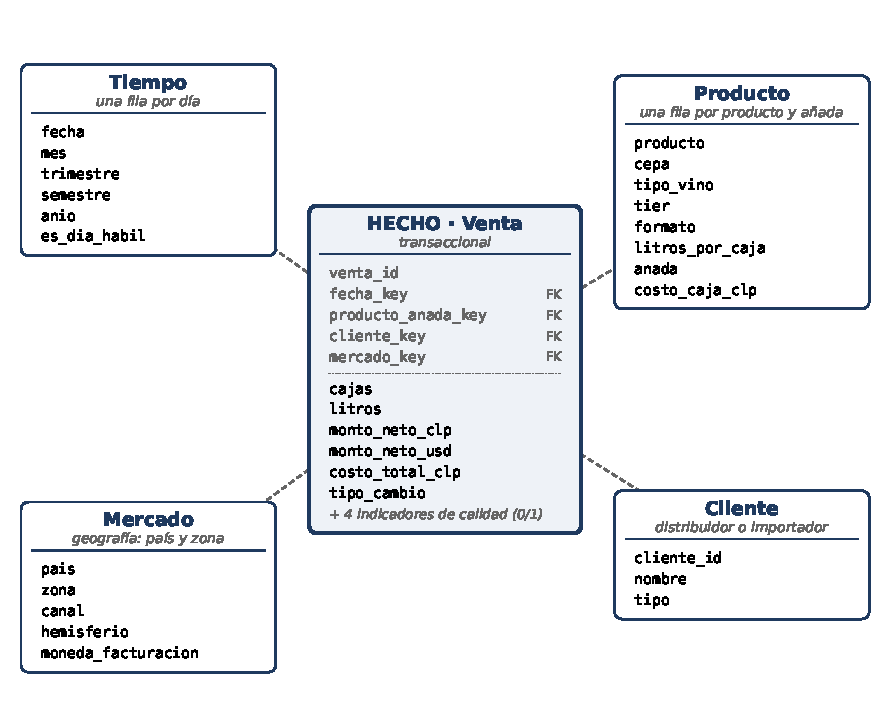
\includegraphics[width=0.66\textwidth]{modelo_estrella.pdf}
  \caption{Modelo estrella de la venta. Fuente: elaboración propia a partir de las cuatro fuentes del caso. Diccionario de datos en el anexo C.}
  \label{fig:modelo}
\end{figure}

Toda cifra del informe se calcula sumando filas de \texttt{fact\_venta}; ninguna sale de una tabla preagregada. De sus \porconfirmar{13.845} filas, \porconfirmar{10.672} son exportaciones de 2025 y forman el universo de la métrica (sección D).

\paragraph{Por qué este grano.} No existe en la fuente un nivel más fino que la línea de venta, y uno más grueso destruye la pregunta: para separar el efecto precio del efecto mezcla, cada fila tiene que conservar su tier y sus litros. Si agregáramos, por ejemplo, por mes y mercado, la mezcla quedaría fija dentro de cada agregado.

\paragraph{El precio por litro no se guarda.} El hecho guarda cajas, litros y montos, que se suman. El precio medio por litro es un indicador, la suma del monto neto dividida por la suma de los litros, y una razón de sumas no es aditiva: se calcula en cada corte, nunca se promedia. Esta decisión es también la respuesta de negocio: como es una razón, el precio por litro sube cuando crece la proporción de litros de los tiers caros, aunque no se mueva ningún precio de lista.

\paragraph{Producto al nivel de producto y añada.} El costo por caja depende del tier y de la añada, así que \texttt{dim\_producto} tiene una fila por producto y añada (\porconfirmar{96}): el costo unitario es atributo de la dimensión y el costo total es hecho. Ahí vive también \texttt{litros\_por\_caja}, de modo que la definición de caja a litro (sección D) es una sola columna y su sensibilidad se calcula cambiando ese atributo. La cepa, escrita con alias distintos en el archivo de costos, se conforma al catálogo de cepas del ERP.

\paragraph{Montos en dos monedas.} La exportación se factura en dólares y el mercado nacional en pesos. Para no sumar pesos con dólares, cada monto se guarda en dos columnas, convertidas con el dólar observado de la fecha de factura. La moneda no va como texto en el hecho: la determina el mercado, así que es atributo de \texttt{dim\_mercado}.

\paragraph{Qué quedó fuera.}

\begin{center}
\small
\begin{tabular}{@{}>{\raggedright\arraybackslash}p{0.24\textwidth}>{\raggedright\arraybackslash}p{0.68\textwidth}@{}}
\toprule
Qué & Por qué \\
\midrule
Embarque (JSON) & Es otro proceso, con su propio grano (un embarque agrupa varias líneas), y su vínculo con la venta no es confiable. La cadena lo usa para corregir cajas cargadas en botellas; queda como la siguiente estrella (anexo C). \\
Vendedor & Redundante: los cinco vendedores corresponden uno a uno a las cinco zonas. \\
RUT del cliente & No aporta a la pregunta; minimización de datos personales. \\
Flete, seguro, aranceles & No están en ninguna fuente. \\
Cobranza & Otro proceso, sin fechas de pago. \\
\bottomrule
\end{tabular}
\end{center}

\paragraph{Qué resuelve y qué no.} El modelo separa precio de mezcla, convierte sin mezclar monedas y costea según la añada. No resuelve el margen por mercado (faltan flete y aranceles), el efecto cambiario real (cobranza a 60 y 90 días, pago en euros) ni si el alza de la gran reserva es estacional: con un año de datos permite el corte mensual, pero no comparar un año con otro.
